\documentclass{article}%
\usepackage{amsmath}%
\usepackage{amsfonts}%
\usepackage{amssymb}%
\usepackage{graphicx}
\usepackage{fancyhdr}
\usepackage{enumitem} % for custom labels
\usepackage{multicol}
\usepackage{xcolor} % For custom colors
\usepackage{hyperref} % For colored references (must be loaded LAST)
\hypersetup{
    colorlinks=true,
    linkcolor=blue, % Color for \ref
    citecolor=blue, % Color for \cite
    urlcolor=blue   % Color for \url
}
\usepackage{tikz}
\usetikzlibrary{shapes,arrows,positioning,intersections}
% Define colors with opacity
\colorlet{setIcolor}{red!30}
\colorlet{setIIcolor}{blue!30}
\colorlet{setIIIcolor}{green!30}
\colorlet{resultcolor}{orange!50}
%-------------------------------------------
\newtheorem{theorem}{Theorem}
\newtheorem{acknowledgement}[theorem]{Acknowledgement}
\newtheorem{algorithm}[theorem]{Algorithm}
\newtheorem{axiom}[theorem]{Axiom}
\newtheorem{case}[theorem]{Case}
\newtheorem{claim}[theorem]{Claim}
\newtheorem{conclusion}[theorem]{Conclusion}
\newtheorem{condition}[theorem]{Condition}
\newtheorem{conjecture}[theorem]{Conjecture}
\newtheorem{corollary}[theorem]{Corollary}
\newtheorem{criterion}[theorem]{Criterion}
\newtheorem{definition}[theorem]{Definition}
\newtheorem{example}[theorem]{Example}
\newtheorem{exercise}[theorem]{Exercise}
\newtheorem{lemma}[theorem]{Lemma}
\newtheorem{notation}[theorem]{Notation}
\newtheorem{problem}[theorem]{Problem}
\newtheorem{proposition}[theorem]{Proposition}
\newtheorem{remark}[theorem]{Remark}
\newtheorem{solution}[theorem]{Solution}
\newtheorem{summary}[theorem]{Summary}
\newenvironment{proof}[1][Proof]{\textbf{#1.} }{\ \rule{0.5em}{0.5em}}
\setlength{\textwidth}{7.0in}
\setlength{\oddsidemargin}{-0.35in}
\setlength{\topmargin}{-0.5in}
\setlength{\textheight}{9.0in}
\setlength{\parindent}{0.3in}
\setlength{\headheight}{22.43335pt}

\usepackage{titlesec}

% Customize section title size and spacing
\titleformat{\section}{\large\bfseries}{\thesection}{1em}{}
\titlespacing{\section}{0pt}{14pt}{8pt}

\titleformat{\subsection}{\large\bfseries}{\thesubsection}{1em}{}
\titlespacing{\subsection}{0pt}{10pt}{6pt}  % Adjust spacing (before/after)

\pagestyle{fancy}
\fancyhf{}
\rhead{Julio 31, 2025}
\chead{Probabilidad \& Estadística }
\lhead{Saul Axel López Gómez}
\rfoot{ \thepage}

\begin{document}


\begin{Large}
\begin{center}
\textbf{Operaciones con Conjuntos y Diagramas de Venn} \\
\end{center}
\end{Large}

\vspace{0.2in}

\begin{small}
    \section*{A partir del universo y subconjuntos, encontrar por extensión y graficar los diagramas de Venn los siguientes incisos} \textit{}
\end{small}

\vspace{0.2in}

Sea: 

\begin{itemize}
    \item U = \{X $\in$ letras del abecedario \} \hspace{0.20in} Nota: No se incluye "ñ" ni "LL"
    \item I = \{X $\in$ vocales \}
    \item II = \{X = h; $\quad$ X = j; $\quad$ o $<$ X $\leq$ s  \}
    \item III = \{a $\leq$ X $<$ k; $\quad$  X = o; $\quad$ X = u  \}
     \item IV = \{f $\leq$ X $<$ i; $\quad$ j $\leq$ X $<$ o $\quad$  p $\leq$ X $\leq$ s \}
\end{itemize}

\vspace{0.10in}

Hallar por extensión y generar el diagrama de Venn para cada caso:

\begin{enumerate}[label=\alph*)]
    \item (I - II') $\cup$ (III' $\cap$ II)'     \label{a}
    \item (II $\cap$ III) - (IV' $\cup$ I')         \label{b}
    \item (III $\cup$ II) $\cap$ (II' $\cap$ IV)'   \label{c}
    \item (II $\cap$ III)' $\cap$ (I $\cup$ II')'   \label{d}
    \item (III $\cup$ II)' $\cap$ (II' $\cap$ I)'    \label{e}
    \item (III' $\cup$ II') $\cap$ (II' $\cap$ I)' - (IV' - III)   \label{f}
\end{enumerate}

\vspace{0.4in}

\textbf{Solución:} 
\vspace{0.3in}

Como primer paso se debe de encontrar todos los subconjuntos y sus complementos, por lo tanto quedan como:


\begin{itemize}
    \item U = \{ a, b, c, d, e, f, g, h, i, j, k, l, m, n, o, p, q, r, s, t, u, v, w, x, y, z \} 
\end{itemize}


\begin{itemize}

    \item I = \{a, e, i, o, u\}
    \item I' = \{ b, c, d, f, g, h, j, k, l, m, n, p, q, r, s, t, v, w, x, y, z \} 

    \item II = \{ h, j, p, q, r, s  \}
    \item II' = \{ a, b, c, d, e, f, g, i, k, l, m, n, o, t, u, v, w, x, y, z \} 

    \item III = \{ a, b, c, d, e, f, g, h, i, j, o, u  \}       
    \item III' = \{ k, l, m, n, p, q, r, s, t, v, w, x, y, z \}

    \item IV = \{ f, g, h, j, k, l, m, n, p, q, r, s  \}
    \item IV' = \{ a, b, c, d, e, i, o, t, u, v, w, x, y, z \} 

\end{itemize}

%%%%%%%%%%%%%%%%%%%%%%%%%%%%%%%%%%%%%%%%%%%%%%%%%%%%%%%%%%%%%%%%%%%%%%%%%%%
\newpage


\textbf{a)} Analizando paso por paso el primer inciso \ref{a}, se puede resolver en dos partes \textbf{(I - II')} y \textbf{(III' $\cap$ II)'} para así unir ambos subconjuntos \\

Resolviendo \textbf{(I - II')}

\begin{align*}
(I - I')  &= \{a, e, i, o, u\} - \{ a, b, c, d, e, f, g, i, k, l, m, n, o, t, u, v, w, x, y, z \}  \\
  &= \{\} \\
\end{align*}

Resolviendo \textbf{(III' $\cap$ II)'}

\begin{align*}
(III' \cap II)'  &= \{ k, l, m, n, p, q, r, s, t, v, w, x, y, z \} \cap (\{ h, j, p, q, r, s  \})'  \\
  &= (\{p, q, r, s \} )'\\
\end{align*}

Juntando ambos lados para armar (I - II') $\cup$ (III' $\cap$ II)':

\begin{align*}
(I - II') \cup (III' \cap II)' &= ( \{ \} \cup \{p, q, r, s \} )' \\
  &= \{p, q, r, s \}' \\
  &= \{ a, b, c, d, e, f, g, h, i, j, k, l, m, n, o, t, u, v, w, x, y, z \} 
\end{align*}

Por lo tanto el resultado es

\begin{equation*}
    \boxed{(I - II') \cup (III' \cap II)' = \{ a, b, c, d, e, f, g, h, i, j, k, l, m, n, o, t, u, v, w, x, y, z \} }
\end{equation*}

Para obtener el diagrama de Venn, se puede hacer por partes, el lado derecho y lado izquierdo, quedando: \\

\textbf{(I - II')}: 

\begin{figure}[htbp]
\centering
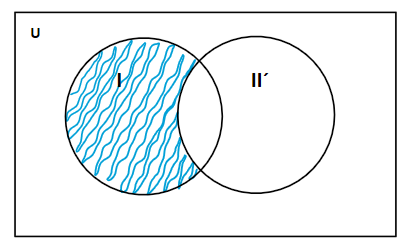
\includegraphics[width=8cm]{a/aa.png}
\caption[]{Diagrama de Venn de (I - II')}
\end{figure} 

\newpage

\textbf{(III' $\cap$ II)'}:

\begin{figure}[htbp]
\centering
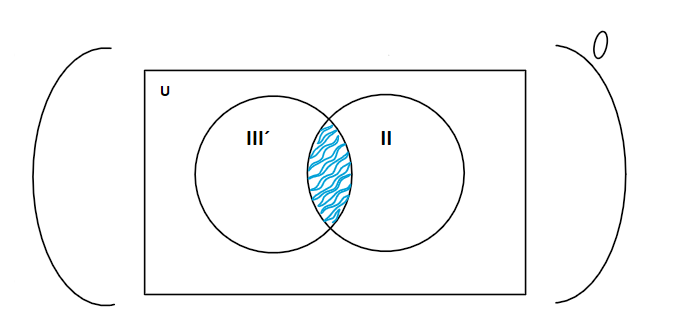
\includegraphics[width=8cm]{a/bb.png}
\caption[]{Diagrama de Venn de (III' $\cap$ II)'}
\end{figure} 

Sacando el complemento, queda el diagrama

\begin{figure}[htbp]
\centering
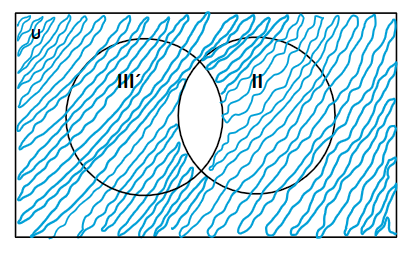
\includegraphics[width=8cm]{a/bbb.png}
\caption[]{Diagrama de Venn de (III' $\cap$ II)'}
\end{figure} 

Haciendo la unión de ambos lados para armar (I - II') $\cup$ (III' $\cap$ II)', quedando así el diagrama de Venn:

\begin{figure}[htbp]
\centering
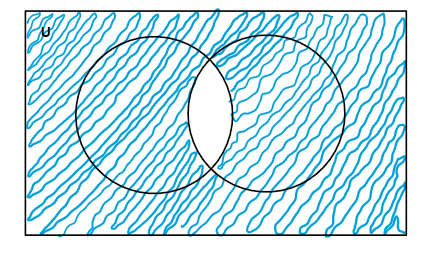
\includegraphics[width=8cm]{a/aabb.png}
\caption[]{Diagrama de Venn de (I - II') $\cup$ (III' $\cap$ II)'}
\end{figure} 
\newpage

%
\textbf{b)} Analizando paso por paso el segundo inciso \ref{b}, se puede resolver en dos partes \textbf{(II $\cap$ III)} y \textbf{(IV' $\cup$ I')} para así unir ambos subconjuntos \\

Resolviendo \textbf{(II $\cap$ III)}

\begin{align*}
(II \cap III)  &= \{ h, j, p, q, r, s  \} \cap \{ a, b, c, d, e, f, g, h, i, j, o, u  \}  \\
  &=   \{ h, j  \}      \\
\end{align*}

Resolviendo \textbf{(IV' $\cup$ I')}

\begin{align*}
(IV' \cup I')  &=  \{ a, b, c, d, e, i, o, t, u, v, w, x, y, z \}  \cup \{ b, c, d, f, g, h, j, k, l, m, n, p, q, r, s, t, v, w, x, y, z \}  \\
  &=  \{ a, b, c, d, e, f, g, h, i, j, k, l, m, n, o, p, q, r, s, t, u, v, w, x, y, z \} \\
\end{align*}

Juntando ambos lados para armar (II $\cap$ III) - (IV' $\cup$ I'):

\begin{align*}
(II \cap III) - (IV' \cup I') &= \{ h, j  \} - \{ a, b, c, d, e, f, g, h, i, j, k, l, m, n, o, p, q, r, s, t, u, v, w, x, y, z \} \\
  &= \{ \} 
\end{align*}

Por lo tanto el resultado es un subconjunto vacío:

\begin{equation*}
    \boxed{(I - I') \cup (III' \cap II)' = \{  \} }
\end{equation*}





Para obtener el diagrama de Venn, se puede hacer por partes, el lado derecho y lado izquierdo, quedando: \\

\textbf{(II $\cap$ III)}: 

\begin{figure}[htbp]
\centering
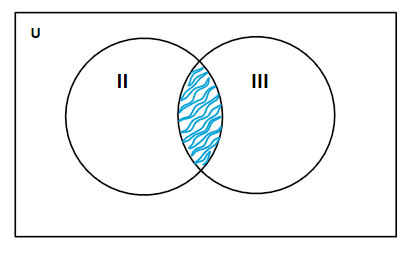
\includegraphics[width=8cm]{b/aa.png}
\caption[]{Diagrama de Venn de (II $\cap$ III)}
\end{figure} 

\newpage

\textbf{(IV' $\cup$ I')}:

\begin{figure}[htbp]
\centering
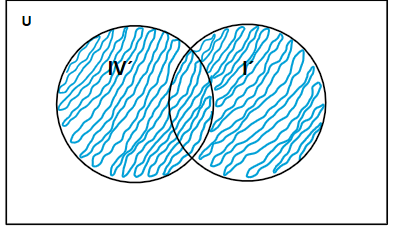
\includegraphics[width=8cm]{b/bb.png}
\caption[]{Diagrama de Venn de (IV' $\cup$ I')}
\end{figure} 

Sacando la diferencia, (II $\cap$ III) - (IV' $\cup$ I'), queda que no existe ningún diagrama representativo, ya que es un subconjunto vacío




\newpage

%   (III $\cup$ II) $\cap$ (II' $\cap$ IV)'
\textbf{c)} Analizando paso por paso el segundo inciso \ref{c}, se puede resolver en dos partes \textbf{(III $\cup$ II)} y \textbf{((II' $\cap$ IV)')} para asi unir ambos subconjuntos \\

Resolviendo \textbf{(III $\cup$ II)}

\begin{align*}
(III \cup II)  &= \{ a, b, c, d, e, f, g, h, i, j, o, u  \}   \cup \{ h, j, p, q, r, s  \} \\
  &=  \{ a, b, c, d, e, f, g, h, i, j, o, p, q, r, s, u  \}        \\
\end{align*}

Resolviendo \textbf{(II' $\cap$ IV)'}

\begin{align*}
(II' \cap IV)'  &=  (\{ a, b, c, d, e, f, g, i, k, l, m, n, o, t, u, v, w, x, y, z \} \cap \{ f, g, h, j, k, l, m, n, p, q, r, s  \} )' \\
  &=  (\{  f, g, k, l, m, n, \} )' \\
  &= \{ a, b, c, d, e, h, i, j, o, p, q, r, s, t, u, v, w, x, y, z \} \\
\end{align*}

Juntando ambos lados para armar (III $\cup$ II) $\cap$ (II' $\cap$ IV)':

\begin{align*}
(III \cup II) \cap (II' \cap IV)' &= \{ a, b, c, d, e, f, g, h, i, j, o, p, q, r, s, u  \} \cap \{ a, b, c, d, e, h, i, j, o, p, q, r, s, t, u, v, w, x, y, z \}\\
  &= \{ a, b, c, d, e, h, i, j, o, p, q, r, s, u \}
\end{align*}

Por lo tanto el resultado es:

\begin{equation*}
    \boxed{ (III \cup II) \cap (II' \cap IV)' =  \{ a, b, c, d, e, h, i, j, o, p, q, r, s, u \}    }
\end{equation*}
\newpage

%   (II $\cap$ III)' $\cap$ (I $\cup$ II')'
\textbf{d)} Analizando paso por paso el segundo inciso \ref{d}, se puede resolver en dos partes \textbf{(II $\cap$ III)'} y \textbf{(I $\cup$ II')'} para asi unir ambos subconjuntos \\

Resolviendo \textbf{(II $\cap$ III)'}

\begin{align*}
 (II \cap III)' &=( \{ h, j, p, q, r, s  \} \cap \{ a, b, c, d, e, f, g, h, i, j, o, u  \}    )'  \\
  &=   (\{ h, j \})'       \\
    &=   \{ a, b, c, d, e, f, g, i, k, l, m, n, o, p, q, r, s, t, u, v, w, x, y, z \}        \\
\end{align*}

Resolviendo \textbf{(I $\cup$ II')'}

\begin{align*}
(I \cup II')'  &=  ( \{a, e, i, o, u\} \cup \{ a, b, c, d, e, f, g, i, k, l, m, n, o, t, u, v, w, x, y, z \}  )'\\
  &=  ( \{ a, b, c, d, e, f, g, i, k, l, m, n, o, t, u, v, w, x, y, z \}  )' \\
  &=       \{h, j, p, q, r, s \}\\
\end{align*}

Juntando ambos lados para armar (II $\cap$ III)' $\cap$ (I $\cup$ II')':

\begin{align*}
(II \cap III)' \cap (I \cup II')' &= \{ a, b, c, d, e, f, g, i, k, l, m, n, o, p, q, r, s, t, u, v, w, x, y, z \} \cap \{h, j, p, q, r, s \} \\
  &= \{p, q, r, s \}
\end{align*}

Por lo tanto el resultado es:

\begin{equation*}
    \boxed{ (II \cap III)' \cap (I \cup II')' =   \{p, q, r, s \}   }
\end{equation*}
\newpage

%   (III $\cup$ II)' $\cap$ (II' $\cap$ I)' 
\textbf{e)} Analizando paso por paso el segundo inciso \ref{e}, se puede resolver en dos partes \textbf{(III $\cup$ II)'} y \textbf{(II' $\cap$ I)' } para asi unir ambos subconjuntos \\

Resolviendo \textbf{(III $\cup$ II)' }

\begin{align*}
(III \cup II)'   &= (\{ a, b, c, d, e, f, g, h, i, j, o, u  \}  \cup \{ h, j, p, q, r, s  \})' \\
  &=    (\{ a, b, c, d, e, f, g, h, i, j, o, p, q, r, s, u, \})'      \\
  &=   \{  k, l, m, n, t, v, w, x, y, z \}      \\
\end{align*}

Resolviendo \textbf{(II' $\cap$ I)' }

\begin{align*}
(II' \cap I)'   &= ( \{ a, b, c, d, e, f, g, i, k, l, m, n, o, t, u, v, w, x, y, z \} \cap \{a, e, i, o, u\} )' \\
  &=    (\{a, e, i, o, u\})'      \\
  &=  \{ b, c, d, f, g, h, j, k, l, m, n, p, q, r, s, t, v, w, x, y, z \}      \\
\end{align*}

Juntando ambos lados para armar (III $\cup$ II)' $\cap$ (II' $\cap$ I)':

\begin{align*}
(III \cup II)' \cap (II' \cap I)'  &= \{  k, l, m, n, t, v, w, x, y, z \} \cap \{ b, c, d, f, g, h, j, k, l, m, n, p, q, r, s, t, v, w, x, y, z \}  \\
  &= \{ k, l, m, n, t,  v, w, x, y, z \}
\end{align*}

Por lo tanto el resultado es:

\begin{equation*}
    \boxed{(III \cup II)' \cap (II' \cap I)'  =   \{ k, l, m, n, t,  v, w, x, y, z \}   }
\end{equation*}
\newpage

%   (III' $\cup$ II') $\cap$ (II' $\cap$ I)' - (IV' - III)
\textbf{f)} Analizando paso por paso el segundo inciso \ref{f}, se puede resolver en tres partes \textbf{} , \textbf{} y \textbf{} para así unir los tres subconjuntos \\

Resolviendo \textbf{(III' $\cup$ II')}

\begin{align*}
(III' \cup II')  &= \{ k, l, m, n, p, q, r, s, t, v, w, x, y, z \} \cup  \{ a, b, c, d, e, f, g, i, k, l, m, n, o, t, u, v, w, x, y, z \} \\
  &=   \{ a, b, c, d, e, f, g, i, k, l, m, n, o, p, q, r, s, t, u, v, w, x, y, z \}       \\
\end{align*}

Resolviendo \textbf{(II' $\cap$ I)' }

\begin{align*}
(II' \cap I)'   &= (\{ a, b, c, d, e, f, g, i, k, l, m, n, o, t, u, v, w, x, y, z \} \cap \{a, e, i, o, u\})' \\
  &=  ( \{a, e, i, o, u\} )' \\
  &= \{ b, c, d, f, g, h, j, k, l, m, n, p, q, r, s, t, v, w, x, y, z \}  \\
\end{align*}


Resolviendo \textbf{(IV' - III)}

\begin{align*}
(IV' - III)  &= \{ a, b, c, d, e, i, o, t, u, v, w, x, y, z \} - \{ a, b, c, d, e, f, g, h, i, j, o, u  \} \\
  &=  \{ t, v, w, x, y, z \}  \\
\end{align*}

Juntando los tres lados para armar (III' $\cup$ II') $\cap$ (II' $\cap$ I)' - (IV' - III):

\begin{align*}
(III' \cup II') \cap (II' \cap I)' - (IV' - III) &= \{ a, b, c, d, e, f, g, i, k, l, m, n, o, p, q, r, s, t, u, v, w, x, y, z \} \\ &\cap \{ b, c, d, f, g, h, j, k, l, m, n, p, q, r, s, t, v, w, x, y, z \}  - \{ t, v, w, x, y, z \}  \\
  &=  \{b, c, d,  f, g, k, l, m, n, p, q, r, s, t, v, w, x, y, z \} 
 - \{ t, v, w, x, y, z \} \\
 &=  \{  b, c, d, f, g, k, l, m, n, p, q, r, s      \} 
\end{align*}

Por lo tanto el resultado es:

\begin{equation*}
    \boxed{(III' \cup II') \cap (II' \cap I)' - (IV' - III)  =  \{  b, c, d, f, g, k, l, m, n, p, q, r, s      \}    }
\end{equation*}


\newpage


Para obtener el diagrama de Venn, se puede hacer por partes, el lado derecho y lado izquierdo, quedando: \\


\textbf{(III' $\cup$ II')}: 

\begin{figure}[htbp]
\centering
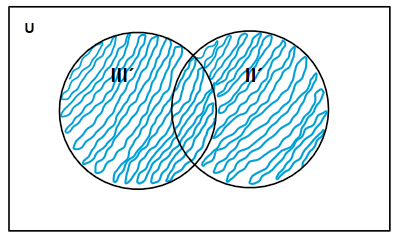
\includegraphics[width=8cm]{f/aa.png}
\caption[]{Diagrama de Venn de (III' $\cup$ II')}
\end{figure} 


\textbf{(II' $\cap$ I)'}:

\begin{figure}[htbp]
\centering
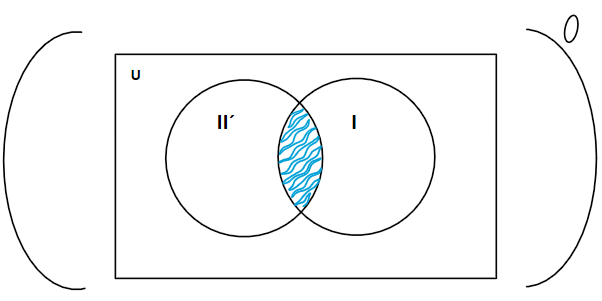
\includegraphics[width=8cm]{f/bb.png}
\caption[]{Diagrama de Venn de (II' $\cap$ I)'}
\end{figure} 

Sacando el complemento, queda el diagrama

\begin{figure}[htbp]
\centering
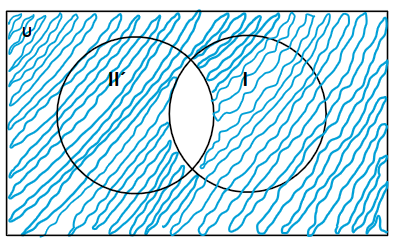
\includegraphics[width=8cm]{f/bbb.png}
\caption[]{Diagrama de Venn de (II' $\cap$ I)'}
\end{figure} 

\newpage

\textbf{(IV' - III)}:

\begin{figure}[htbp]
\centering
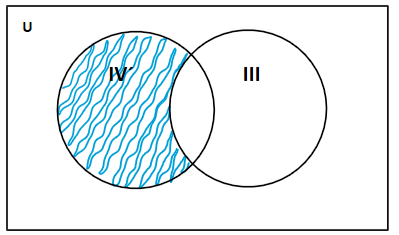
\includegraphics[width=7cm]{f/cc.png}
\caption[]{Diagrama de Venn de (IV' - III)}
\end{figure} 

Haciendo la intersección de (III' $\cup$ II') $\cap$ (II' $\cap$ I)', quedando así:

\begin{figure}[htbp]
\centering
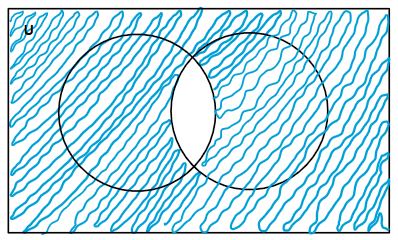
\includegraphics[width=7cm]{f/aabb.png}
\caption[]{Diagrama de Venn de (III' $\cup$ II') $\cap$ (II' $\cap$ I)'}
\end{figure} 


Haciendo la diferencia de (III' $\cup$ II') $\cap$ (II' $\cap$ I)' - (IV' - III), quedando así:

\begin{figure}[htbp]
\centering
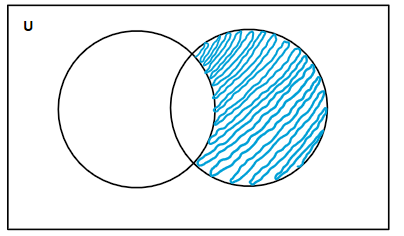
\includegraphics[width=7cm]{f/aabbcc.png}
\caption[]{Diagrama de Venn de (III' $\cup$ II') $\cap$ (II' $\cap$ I)' - (IV' - III)}
\end{figure} 

%%%%%%%%%%%%%%%%%%%%%%%%%%%%%%%%%%%%%%%%%%%%%%%%%%%%%%%%%%%%%%%%%%%%%%%%%%%





\newpage
%%%%%%%%%%%%%%%%%%%%%%%%%%%%%%%%%%%%%%%%%%%%%%%%%%%%%%%%%%%%%%%%%%%%%%%%%%%






\newpage
%%%%%%%%%%%%%%%%%%%%%%%%%%%%%%%%%%%%%%%%%%%%%%%%%%%%%%%%%%%%%%%%%%%%%%%%%%%






\newpage
%%%%%%%%%%%%%%%%%%%%%%%%%%%%%%%%%%%%%%%%%%%%%%%%%%%%%%%%%%%%%%%%%%%%%%%%%%%






\newpage
%%%%%%%%%%%%%%%%%%%%%%%%%%%%%%%%%%%%%%%%%%%%%%%%%%%%%%%%%%%%%%%%%%%%%%%%%%%





\newpage
%%%%%%%%%%%%%%%%%%%%%%%%%%%%%%%%%%%%%%%%%%%%%%%%%%%%%%%%%%%%%%%%%%%%%%%%%%%






\newpage
%%%%%%%%%%%%%%%%%%%%%%%%%%%%%%%%%%%%%%%%%%%%%%%%%%%%%%%%%%%%%%%%%%%%%%%%%%%






\newpage
%%%%%%%%%%%%%%%%%%%%%%%%%%%%%%%%%%%%%%%%%%%%%%%%%%%%%%%%%%%%%%%%%%%%%%%%%%%






\newpage
%%%%%%%%%%%%%%%%%%%%%%%%%%%%%%%%%%%%%%%%%%%%%%%%%%%%%%%%%%%%%%%%%%%%%%%%%%%






\newpage
%%%%%%%%%%%%%%%%%%%%%%%%%%%%%%%%%%%%%%%%%%%%%%%%%%%%%%%%%%%%%%%%%%%%%%%%%%%






\newpage
%%%%%%%%%%%%%%%%%%%%%%%%%%%%%%%%%%%%%%%%%%%%%%%%%%%%%%%%%%%%%%%%%%%%%%%%%%%







\end{document}